\classheader{Lecture 10}
\setcounter{lecture}{10}
\begin{center}
	\Large \bf Integration: Measurable and Simple Functions
\end{center}
\vspace{0.25cm}

We now assume given $\left( {\Omega ,\mathcal{F},\mu } \right)$ where $\Omega$ is a space, $\mathcal{F}$ a $\sigma-$field of subsets of $\Omega$ and $\mu$ a measure on $\mathcal{F}$.


Before defining such an operator $\mathcal{I}$, we examine the sort of properties $\mathcal{I}$ should have before we would be justified in calling it an integral. Suppose that $\mathcal{A}$ is a class of functions $f:\Omega  \to \overline {\mathbb{R}} $, and $\mathcal{I}:\mathcal{A} \to\mathbb{R}$ defines a real number for every $ f \in \mathcal{A} $. Then we want $\mathcal{I}$ to satisfy:
\begin{enumerate}
	\item $f \in \mathcal{A},f\left( x \right) \geqslant 0,$ all $ x \in \Omega  \Rightarrow \mathcal{I}\left( f \right) \geqslant 0$, that is $\mathcal{I}$ preserves positivity 
	\item $f,g\; \in {\mathcal{A}},\;\alpha  \in \mathbb{R} \Rightarrow \alpha f + g \in \mathcal{A}$ and
	\begin{equation}
	\mathcal{I}\left( {\alpha f + g} \right) = \alpha \mathcal{I}\left( f \right) + \mathcal{I}\left( g \right)
	\end{equation}
	that is $\mathcal{I}$ is linear on $\mathcal{A}$.
	\item $\mathcal{I}$ is continuous on $\mathcal{A}$ in some sense, at least we would want to have $\mathcal{I}\left( {{f_n}} \right) \to 0$ as $ n \to \infty $ for any sequence decreasing with ${f_n}\left( x \right) \to 0$ for all $ x $ in $\Omega$.
\end{enumerate}

These conditions are satisfied by the elementary integration process, but the Riemann integral does not satisfy the following strengthened form of $ 3 $.

\begin{itemize}
	\item  $ 3^{\prime} $ If $\left\{ {{f_n}} \right\}$ is an increasing sequence of functions in $\mathcal{A}$, and 
	\begin{equation}
	{f_n}\left( x \right) \to f\left( x \right)\;\;for\;\;all\;\;x \in \Omega 
	\end{equation}
	then $ f \in \mathcal{A} $ and $\mathcal{F}\left( {{f_n}} \right) \to \mathcal{F}\left( f \right)\;as\;n \to \infty $
\end{itemize}
 
    \begin{figure}[!htb]
 	\centering
 	\subfloat[Riemann integral]{
 		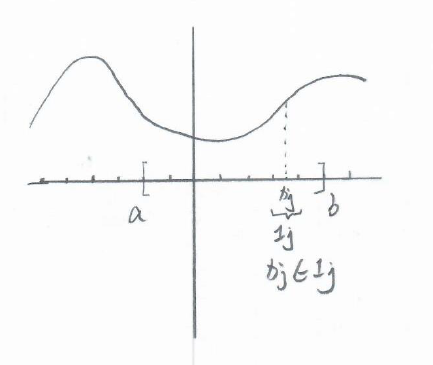
\includegraphics[width=0.3\linewidth,height=0.2\linewidth]{fig101.png}}
 	\label{img101}\qquad \qquad 
 	\subfloat[Lebesgue integration]{
 		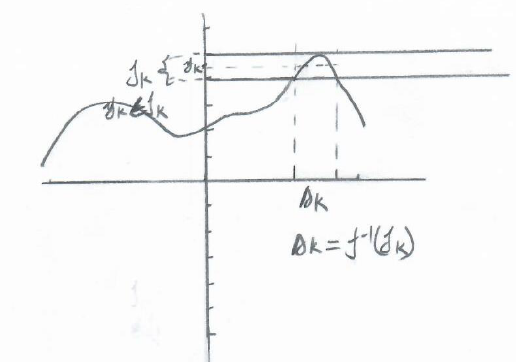
\includegraphics[width=0.3\linewidth,height=0.2\linewidth]{fig102.png}}
 	\label{img102}
 	\caption{Integration}
 \end{figure}

\begin{enumerate}
	\item Riemann integral
	\begin{equation}
	\int f  \approx \sum {f\left( {{x_j}} \right)} \left| {{I_j}} \right|
	\label{eq10.3}
	\end{equation}
	\item Lebesgue integration
	\begin{equation}
	I\left( f \right) \approx \sum {{y_k}\mu \left( {{A_k}} \right)}  = \sum\limits_k {{y_k}\mu \left( {{f^{ - 1}}\left( {{J_k}} \right)} \right)} 
	\end{equation}
	where ${A_k} = {f^{ - 1}}\left( {{J_k}} \right)$.
\end{enumerate}

In defining measurability we will want to consider functions
\begin{equation}
f:\Omega  \to \mathbb{R} \cup \left\{ { - \infty ,\infty } \right\} = \overline {\mathbb{R}}
\label{eq10.5}
\end{equation}
It is possible to define the class of Borel sets $\mathcal{B}$ in $ \overline {\mathbb{R}} $ in terms of this topology. However, we adopt the simple procedure of defining the class 
\begin{equation}
\overline {\mathcal{B}}  = \left\{ {A \cup B,A \in {\mathcal{B}},B \subseteq \left\{ { - \infty ,\infty } \right\}} \right\}
\label{eq10.6}
\end{equation}

\begin{proposition}
	$ \overline {\mathcal{B}} $ is a$ \sigma $-algebra.
\end{proposition}

\begin{definition}
	A function $f:\Omega  \to \overline {\mathbb{R}} $ is said to be $\mathcal{F}-$measurable if and only if 
	\begin{equation}
	{f^{ - 1}}\left( A \right) \in \mathcal{F}
	\end{equation}
	for all $A \in \overline {\mathcal{B}} $.
	\label{def10.1}
\end{definition}

If there is only one $\sigma-$field $\mathcal{F}$ under discussion we may say that $ f $ is a measurable function.

{\color{red} 
	\begin{remark}
		\begin{equation}
		\mathcal{F} \subseteq \mathcal{G}
		\end{equation}
	\end{remark}

}

\begin{lemma}
	$\left( {\Omega ,\mathcal{F},\mu } \right)\;f:\Omega  \to \overline {\mathbb{R}} $, $ f $ is measurable each of the following conditions is necessary and sufficient:
	\begin{enumerate}
		\item ${f^{ - 1}}\left( {\left( { - \infty ,x} \right]} \right) \in \mathcal{F},\;\forall x \in \mathbb{R},\; i.e. \; \left\{ {\omega  \in \Omega ,f\left( \omega  \right) \leqslant x} \right\} \in \mathcal{F} $
		\item ${f^{ - 1}}\left( {\left( { - \infty ,x} \right)} \right) \in \mathcal{F},\;\forall x \in \mathbb{R},\; i.e. \; \left\{ {\omega  \in \Omega ,f\left( \omega  \right) < x} \right\} \in \mathcal{F}$
		\item ${f^{ - 1}}\left( \left[ {x,\infty } \right) \right) \in \mathcal{F},\;\forall x \in \mathbb{R},\; \;  i.e. \; \left\{ {\omega  \in \Omega ,f\left( \omega  \right) \ge x} \right\} \in \mathcal{F} $
		\item ${f^{ - 1}}\left( {\left( { x, \infty} \right)} \right) \in \mathcal{F},\;\forall x \in \mathbb{R},\; \; i.e. \; \left\{ {\omega  \in \Omega ,f\left( \omega  \right) > x} \right\} \in \mathcal{F}$
	\end{enumerate}
\label{lma10.1}
\end{lemma}

\begin{proof}
	We only proof (1) in Lemma \ref{lma10.1} 
	\begin{enumerate}
		\item $ \Rightarrow $ $ \left( { - \infty ,x} \right] \in \overline {\mathcal{B}} $ 
		\item $ \Leftarrow $ If we suppose that the condition is satisfied, and put
		\begin{equation}
		\mathcal{C} = \left\{ {A \in \overline {\mathcal{B}} ,{f^{ - 1}}\left( A \right) \in {\mathcal{F}}} \right\}
		\label{eq10.9}
		\end{equation}
		then
		\begin{enumerate}
			\item $ \mathcal{C} $ is a $ \sigma $-algebra 
			\item $ \mathcal{C} \supseteq\mathcal{G} = \left\{ {\left( { - \infty ,x} \right],x \in \mathbb{R}} \right\} $
		\end{enumerate}
	by $ a\&b $ ,
	\begin{equation}
	\mathcal{C} \supseteq \mathcal{F}\left( \mathcal{G} \right) \supseteq \overline {\mathcal{B}} 
	\label{eq10.10}
	\end{equation}
	then $ \mathcal{C} $ is a $ \sigma $-algebra.
	\begin{itemize}
		\item $\overline {\mathbb{R}}  \in \mathcal{C},{f^{ - 1}}\left( {\overline {\mathbb{R}} } \right) = \left\{ {\omega  \in \Omega ,f\left( \omega  \right) \in \overline {\mathbb{R}} } \right\} = \Omega  \in {\mathcal{F}}$
		\item $ A \in \mathcal{C} \Rightarrow A^{c} \in \mathcal{C}, {f^{ - 1}}\left( A \right) \in \mathcal{F} $, so ${f^{ - 1}}\left( {{A^c}} \right) \in {f^{ - 1}}{\left( A \right)^c} \in \mathcal{F}$
		\item ${A_j} \in \mathcal{C} \Rightarrow \bigcup\limits_{j \geqslant 1} {{A_j}}  \in \mathcal{C}$, then
		\begin{equation}
		{f^{ - 1}}\left( {\bigcup\limits_{j \geqslant 1} {{A_j}} } \right) = \bigcup\limits_j {\;\underbrace {{f^{ - 1}}\left( {{A_j}} \right)}_{ \in {\mathcal{F}}}}  \in {\mathcal{F}}
		\label{eq10.11}
		\end{equation}
	\end{itemize}	
	\end{enumerate}
%	\begin{enumerate}
%		\setcounter{enumi}{5}
%		\item $ \mathcal{C} $ is a $ \sigma $-algebra 
%		\item $ \mathcal{C} \supseteq\mathcal{G} = \left\{ {\left( { - \infty ,x} \right],x \in \mathbb{R}} \right\} $
%    \end{enumerate}
\end{proof}

Given $\left( {\Omega ,\mathcal{F},\mu } \right)$ as above. If $\Omega  = \bigcup\limits_{i = 1}^n {{E_i}} $ and the sets $ E_{i} $ are disjoint (${E_j} \cap {E_k} = \emptyset ,\;j \ne k$), then $ E_{1},E_{2},...,E_{n} $ are said to form a (finite) dissection of $ \Omega $. They are said to form an $ \mathcal{C} $-dissection if, in addition $ E_{i} \in \mathcal{F}(i=1,2,...,n) $.

\begin{definition}[Simple Function]
	A function $f:\;\Omega  \to \mathbb{R}$ is called $ \mathcal{F} $-simple if it can be expressed as
	\begin{equation}
	f = \sum\limits_{j = 1}^n {{c_j}\;{1_{{E_j}}}} ,\;{c_j} \in \mathbb{R}
	\label{eq10.12}
	\end{equation}
	where $ 1_{E_{j}}, \Omega  \to \overline {\mathbb{R}}$,
	\begin{equation}
	\omega  \mapsto {1_{{E_j}}}\left( \omega  \right) = \left\{ {\begin{matrix}
		{1,}  \\ 
		{0,}  \\ 
		
		\end{matrix} } \right.\;\begin{matrix}
	{\omega  \in {E_j}}  \\ 
	{\omega  \notin {E_j}}  \\ 
	
	\end{matrix}
	\label{eq10.13} 
	\end{equation}
	\label{def10.2}
	and $\sum\limits_{j = 1}^n {{E_j}}  = \Omega ,\;{E_0} = \Omega \backslash \left( {\sum\limits_{j = 1}^n {{E_j}} } \right) \in \mathcal{F}$.
\end{definition}

If there is only one $\sigma-$field $\mathcal{F}$ under discussion we will talk of simple function rather than $ \mathcal{F} $-simple functions.

${f^{ - 1}}\left( A \right) = \sum\limits_{k,{c_k}} {{E_k}}  \in {\mathcal{F}},\;A \in \overline {\mathcal{B}},$ $f:\Omega  \to R{}_ + ,\;f = \sum\limits_{j = 1}^n {{c_j}{1_{{E_j}}}} ,\;{E_j} \in {\mathcal{F}},\;\left\{ {{E_1},...,{E_n}} \right\}\;partition\;of\;\Omega $.

\begin{figure}[!htb]
	\centering
	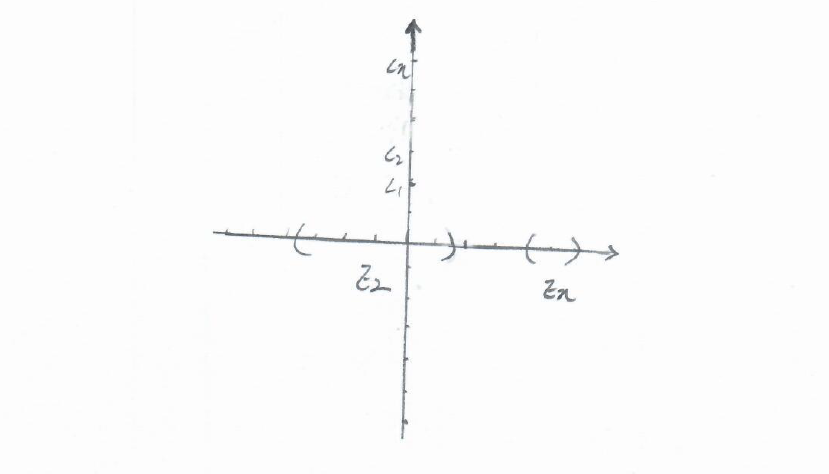
\includegraphics[width=0.6\linewidth,height=0.2\linewidth]{/fig103.png}
	%\caption{Unfolding of recurrency}
\end{figure}

\begin{equation}
I\left( f \right) = \sum\limits_{j = 1}^n {{c_j}\mu \left( {{E_j}} \right)} 
\label{eq10.14}
\end{equation}
where ${c_j} \geqslant 0$.

If $f = \sum\limits_{k = 1}^m {{d_k}{1_{{F_k}}}} $.

\begin{proposition}
	${E_{{j^ \circ }}} \cap {F_{{k^ \circ }}} \ne \emptyset $, then 
	\begin{equation}
	\sum\limits_{j = 1}^n {{c_j}\mu \left( {{E_j}} \right)}  = \sum\limits_{k = 1}^n {{d_k}\mu \left( {{F_k}} \right)} 
	\end{equation}
	\label{prop10.2}
\end{proposition}

\begin{proof}
	\begin{equation}
	\begin{split}
	\mu \left( {{E_j}} \right) & = \mu \left( {{E_j} \cap \left( {\sum\limits_{k = 1}^m {{F_k}} } \right)} \right)\\
							   & = \mu \left( {\sum\limits_{k = 1}^m {{{\left( {{E_j} \cap F_{k}} \right)}}} } \right)\\
							   & = \mu \left( {{E_j}} \right) = \sum\limits_{k = 1}^m {\mu \left( {{E_j} \cap {F_k}} \right)}
	\end{split}
	\label{eq10.16}
	\end{equation}
	then
	\begin{equation}
	\begin{split}
	\sum\limits_{j = 1}^n {{c_j}\mu \left( {{E_j}} \right)} & = \sum\limits_{j = 1}^n {\sum\limits_{k = 1}^m {{c_j}\mu \left( {{E_j} \cap {F_k}} \right)} } \\
															&  = \sum\limits_{j = 1}^n {\sum\limits_{k = 1}^m {{d_k}\mu \left( {{E_j} \cap {F_k}} \right)} } \\
															& = \sum\limits_{k = 1}^m {{d_k}\mu \left( {{F_k}} \right)} 
	\end{split}
	\end{equation}
\end{proof}

\begin{proposition}
	\text{}
	\begin{enumerate}
		\item $f:\;\Omega  \to {\overline {\mathbb{R}} _ + }$ measurable then there exists ${\left( {{f_n}} \right)_{n \geqslant 1}},\;{f_n}$ simple functions, such that ${f_n} \geqslant 0,\;{f_n} \uparrow f$
		\item $I\left( f \right) = \mathop {\lim }\limits_n \;I\left( {{f_n}} \right)$
		\item $f:\;\Omega  \to \overline {\mathbb{R}} $ measurable, ${f^ + } = \max \left( {f,0} \right),\;{f^ - } = \max \left( { - f,0} \right),\;{f^ + },{f^ - }$ measurable then $f = {f^ + } - {f^ - }$, then 
		\begin{equation}
		I\left( f \right) = I\left( {{f^ + }} \right) - I\left( {{f^ - }} \right)
		\label{eq10.18}
		\end{equation}
	\end{enumerate}
	\label{prop10.3}
\end{proposition}

\begin{example}
	$\Omega  = \left( {0,1} \right],\;{\mathcal{B}},\lambda ,\;\;E = \mathbb{Q} \cap \Omega ,\;f = {1_{{E^c}}}\;$, i.e.  $ f $ simple, then
	\begin{equation}
	I\left( f \right) = \lambda \left( {{E^c}} \right) = 1
	\label{eq10.19}
	\end{equation} 
\end{example}